% Yeban User Guide — Chapter 2: Projects (English)
% T-DOC-001 chapter-by-chapter delivery. Same structure as the Chinese chapter.
% Sources: app.slint menus, host.rs project/template/chooser wiring,
% startup_chooser.rs NewProjectDetails, docs/manual/02-projects.md.

\chapter{Projects}
\label{ch:projects}

This chapter covers the whole project lifecycle: how to create, open, save and reuse
a project, plus Yeban's distinctive "undo is versioning" model. By the end you should
be able to save work confidently, find it again, and return to any past state.

\section{Create, Open and Save}

\subsection{Five entries in the File menu}

The File menu has five project-related items:

\begin{itemize}
  \item \textbf{New Empty Project}: a project with only the master bus.
  \item \textbf{New from Template...}: opens the template chooser to start from a factory or user template.
  \item \textbf{Open / Restore Project...}: pick a \texttt{.yeban} file in the file dialog.
  \item \textbf{Save Project (Cmd/Ctrl+S)}: write the current project back to its file.
  \item \textbf{Save As (Cmd/Ctrl+Shift+S)}: save under a different name or location.
\end{itemize}

You can also open directly from the command line: \texttt{yeban-app --open <path>}.

\screenshot{ch02-file-menu}{The File menu expanded, labelling New Empty Project, New from Template, Open/Restore, Save and Save As}

\subsection{The startup project chooser}

When you launch without specifying a project, the startup project chooser appears.
It groups entry points into \textbf{Recent Projects}, \textbf{Demo Projects},
\textbf{Factory Templates}, \textbf{User Templates}, and an empty-project entry left
on the ``New Project'' tab. A demo lets you look around without touching your work;
a recent project returns you to where you left off.

\screenshot{ch02-startup-chooser}{The startup project chooser with its four category tabs and the ``New Project'' tab}

\subsection{Saving is atomic}

Saving is atomic: content is written to a temporary location first and replaces the
target only once it is complete. A power cut mid-write cannot leave a half-written
project — you get either the new version or the previous one.

\begin{figure}[htbp]
\centering
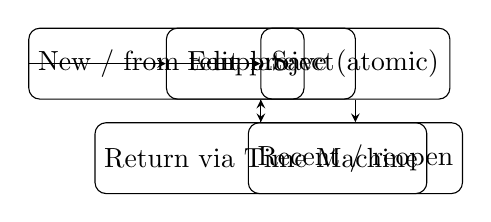
\begin{tikzpicture}[node distance=1.2cm, >=stealth,
    box/.style={draw, rounded corners, align=center, minimum width=2.4cm, minimum height=0.9cm}]
  \node[box] (a) {New / from template};
  \node[box, right of=a] (b) {Edit project};
  \node[box, right of=b] (c) {Save (atomic)};
  \node[box, below of=c] (d) {Recent / reopen};
  \node[box, below of=b] (e) {Return via Time Machine};
  \draw[->] (a) -- (b); \draw[->] (b) -- (c); \draw[->] (c) -- (d);
  \draw[->] (b) -- (e); \draw[->] (e) -- (b);
\end{tikzpicture}
\caption{Project lifecycle: new/from template $\to$ edit $\to$ save $\to$ reopen; you can return to an older version at any time}
\label{fig:ch02-lifecycle}
\end{figure}

\section{Project Files and the Asset Pool}

A project uses the \texttt{.yeban} extension and is the only project format. One
container holds tracks, clips, notes, device chains, and the materials the project
uses (kept in the asset pool, addressed by content hash).

The asset pool means "the project brings its own materials": copy a project to
another machine and the audio and SFZ samples it uses travel with the container.
Stem export and Save As Template both take the pool from the same source, matching
the CLI and MCP behaviour (see Chapter 8).

\begin{table}[htbp]
\centering
\caption{Where things live inside a project}
\label{tab:ch02-container}
\begin{tabular}{ll}
\hline
Content & Location in the project \\
\hline
Tracks / clips / notes & Arrangement data \\
Device chains & The device sequence of each track \\
History DAG & The undo chain, saved with the project \\
Used materials & Asset pool, addressed by content hash \\
Project settings & Tempo / key / time signature / sample rate \\
\hline
\end{tabular}
\end{table}

\section{Templates: New from Template, Save As, Factory Directory}

\subsection{New from template}

File $\to$ New from Template... opens the template chooser, listing two kinds:
\textbf{factory templates} (shipped with the app) and \textbf{user templates} (ones
you saved). Selecting one creates a new project from that skeleton. When the list is
long, the chooser reports the number of hidden rows rather than silently dropping
entries.

\subsection{Save as template}

File $\to$ Save As Template... opens a dialog: enter a name, then confirm to write
into the user template directory. If a template with that name already exists, the
app does not overwrite it directly — it stops and asks for confirmation; cancelling
writes nothing. The user template directory is created on first use; if it is
unavailable, the dialog shows the error rather than failing silently.

\screenshot{ch02-template-dialog}{The Save As Template dialog showing the name field, hint line and same-name confirmation state}

\section{Recent Projects and Recovery}

Every successful open records the path in Recent Projects. You find it under the
``Recent Projects'' tab of the startup chooser and open it with one click; the list
also offers a removal entry for records you no longer need. Recent projects, language
and layout share one local settings store, so changing language or layout does not
push recent projects out.

Open / Restore Project... is also used for recovery: after you select a container
file, the app restores the scene from the history DAG and asset pool recorded in it.

\section{Project Settings: Sample Rate, Tempo, Time Signature}

On the ``New Project'' tab of the startup chooser you can set a few basics for the
empty project; they are written into the new project:

\begin{itemize}
  \item \textbf{Tempo (BPM)}: accepted range 20--999; out-of-range or invalid input is folded back into the legal domain.
  \item \textbf{Key signature}: it can be unset (the factory state of a canonical empty project), or use sharps/flats from $-7$ to $+7$.
  \item \textbf{Time signature}: numerator 1--32; denominator only 1, 2, 4, 8, 16 or 32.
  \item \textbf{Sample rate}: the project's audio sample rate (Hz).
\end{itemize}

These drive later conversions: bar length comes from the time signature, and the
timecode grid from the project's time signature. When a time signature is invalid,
the app reports the reason literally (e.g.\ ``invalid time signature, cannot compute
clip length'') instead of quietly substituting a default.

\screenshot{ch02-new-project-details}{The New Project tab showing the four inputs: tempo, key signature, time signature and sample rate}

\section{Undo Is Versioning: the Time Machine}

Yeban has no separate "version history" feature: every edit is a commit, and undo/
redo merely move along that commit chain.

\begin{itemize}
  \item \textbf{Undo}: Cmd/Ctrl+Z; \textbf{Redo}: Cmd/Ctrl+Shift+Z.
  \item \textbf{Time Machine (Undo Tree)}: Edit $\to$ Time Machine (Undo Tree)...; Cmd/Ctrl+Shift+H also opens it.
\end{itemize}

The Time Machine draws the whole commit chain as a graph: click any version node to
return the project to that state. If there are too many older versions to fit, the
panel reports how many were not drawn rather than pretending all are shown. The
history DAG is saved with the project, so it is still there next time you open it.

\screenshot{ch02-undo-tree}{The Undo Tree graph with a historical node selected and highlighted}

\section{Help Topic Mapping}

\begin{table}[htbp]
\centering
\caption{Sections of this chapter $\to$ in-app help anchors}
\label{tab:ch02-help}
\begin{tabular}{ll}
\hline
Section & Help topic \\
\hline
Five entries in the File menu & \texttt{project-file-menu} \\
Startup project chooser & \texttt{project-startup-chooser} \\
Saving is atomic & \texttt{project-atomic-save} \\
Project files and asset pool & \texttt{project-container-assets} \\
New from template & \texttt{project-template-new} \\
Save as template & \texttt{project-template-save} \\
Recent projects and recovery & \texttt{project-recent-recovery} \\
Project settings & \texttt{project-settings} \\
Undo is versioning: Time Machine & \texttt{project-undo-tree} \\
\hline
\end{tabular}
\end{table}

\paragraph{What you will be able to do} Create, open, save and reuse a project, return to any historical version with the Time Machine, and explain what a \texttt{.yeban} container holds.

\paragraph{Hands-on exercise} Create a project from a template, set tempo to 96 BPM and time signature 3/4; save it, then save it as a template; make several edits, undo with Cmd/Ctrl+Z and jump back to the earliest version with the Time Machine; finally quit, reopen from Recent Projects in the startup chooser and verify the settings survived.
